%%%%%%%%%%%%%%%%%%%%%%%%%%%%%%%%%%%%%%%%%
% Short Sectioned Assignment
% LaTeX Template
% Version 1.0 (5/5/12)
%
% This template has been downloaded from:
% http://www.LaTeXTemplates.com
%
% Original author:
% Frits Wenneker (http://www.howtotex.com)
%
% License:
% CC BY-NC-SA 3.0 (http://creativecommons.org/licenses/by-nc-sa/3.0/)
%
%%%%%%%%%%%%%%%%%%%%%%%%%%%%%%%%%%%%%%%%%

%----------------------------------------------------------------------------------------
%	PACKAGES AND OTHER DOCUMENT CONFIGURATIONS
%----------------------------------------------------------------------------------------

\documentclass[paper=a4, fontsize=11pt]{scrartcl} % A4 paper and 11pt font size
\parskip=4pt
\parindent=0pt
%My packages
\usepackage{qtree}
\usepackage{amsmath}
\usepackage{tikz}
\usepackage{tikz-qtree}
\usepackage{graphicx}

\usepackage{wrapfig}
\usepackage[T1]{fontenc} % Use 8-bit encoding that has 256 glyphs
\usepackage{fourier} % Use the Adobe Utopia font for the document - comment this line to return to the LaTeX default
\usepackage[english]{babel} % English language/hyphenation
\usepackage{amsmath,amsfonts,amsthm} % Math packages
\usepackage{graphicx}

\usepackage{lipsum} % Used for inserting dummy 'Lorem ipsum' text into the template

\usepackage{tabularx} % table control

% for subfigures 
\usepackage{graphicx}
\usepackage{caption}
\usepackage{subcaption}

\usepackage{enumerate}

%Float packages
\usepackage{float}
\usepackage{perpage}
\MakeSorted{figure} %if using both float and fixed figues - prefereably don't
\MakeSorted{table} %if using both fixed and float tables. Prefereably don't

\usepackage{sectsty} % Allows customizing section commands
\allsectionsfont{\centering \normalfont\scshape} % Make all sections centered, the default font and small caps

\usepackage{fancyhdr} % Custom headers and footers
\pagestyle{fancyplain} % Makes all pages in the document conform to the custom headers and footers
\fancyhead{} % No page header - if you want one, create it in the same way as the footers below
\fancyfoot[L]{} % Empty left footer
\fancyfoot[C]{} % Empty center footer
\fancyfoot[R]{\thepage} % Page numbering for right footer
\renewcommand{\headrulewidth}{0pt} % Remove header underlines
\renewcommand{\footrulewidth}{0pt} % Remove footer underlines
\setlength{\headheight}{13.6pt} % Customize the height of the header

\numberwithin{equation}{section} % Number equations within sections (i.e. 1.1, 1.2, 2.1, 2.2 instead of 1, 2, 3, 4)
\numberwithin{figure}{section} % Number figures within sections (i.e. 1.1, 1.2, 2.1, 2.2 instead of 1, 2, 3, 4)
\numberwithin{table}{section} % Number tables within sections (i.e. 1.1, 1.2, 2.1, 2.2 instead of 1, 2, 3, 4)

\setlength\parindent{0pt} % Removes all indentation from paragraphs - comment this line for an assignment with lots of text

%----------------------------------------------------------------------------------------
%	TITLE SECTION
%----------------------------------------------------------------------------------------

\newcommand{\horrule}[1]{\rule{\linewidth}{#1}} % Create horizontal rule command with 1 argument of height

\title{	
\normalfont \normalsize 
\textsc{Vision and Image processing,  Assignment 3} \\ [25pt] % Your university, school and/or department name(s)
\horrule{0.5pt} \\[0.4cm] % Thin top horizontal rule
\huge Segmentation: Snakes \\ % The assignment title
\horrule{2pt} \\[0.5cm] % Thick bottom horizontal rule
}

\author{Maria Barrett, dtq912\\Guangliang Liu, bxd337\\Alexander Wahl-Rasmussen, lgv740} % Your name

\date{\normalsize\today} % Today's date or a custom date

\begin{document}

\maketitle % Print the title

\section{Introduction}
This report describes the process of making a snake and experiments with different weights for the energies. 
\

\section{About Snakes}
The Snakes algorithm is an active contour model, which purpose is to identify and correctly mark the edges of an object in a two dimensional image, i.e. image segmentation. As with many other algorithms, the name itself gives us a hint of how it works. Conceptually, we can think of the algorithm as a snake that tries to squeeze a log as tight as possible, where it first surrounds the log and then squeezes it. Mathematically, we can speak of a contour that tries to minimize its energy, as the sum of its internal and external energies, over a set of iterations in scale-space. So how does this come about?
\

Initially, the algorithm is fed an input in the form of a rough outline of the object it is supposed to match. How the input is given is not that important for the algorithm, but the input itself is of great importance, meaning it should be a set of coordinates that denotes a specific object and not multiple objects. The algorithm then performs spline interpolation on the coordinates, which creates multiple new points within the same discrete set of known coordinates by utilizing low polynomials between each coordinate. With this, we have an initial elastic curve which is closed by setting the last coordinate equal to the first. The initial curve is then sought to be molded via energy minimization over the external and internal energies. The internal energy is defined as the force that draws the curve inwards towards a single point. This energy should be lower the closer it gets to the object. The energy level can be controlled by the constants $\alpha$ and $\beta$ and we will later show how these constants affect the internal energies, but for now it will suffice to say that increasing these constants will increase the importance of the internal energies. 
\

In our implementation we only utilize the image gradient to compute the external energies, but other metrics such as the zero-crossing of the Laplacian of Gaussians can likewise be used. Furthermore, it is possible to constrain the energy, as done in the original Snakes implementation in order to control the importance of each energy for each iteration. By using the image gradient we can assume that the external energy will increase as the snake is approaching an edge given that the highest gradient in a Gaussian denotes the top of the Gaussian. We can then change the weight of the external energy by changing the $\gamma$ constant, which effect we will show in the later parts of the reports.
\

\section{Our implementation}
To a large extent we use Francois' provided functions. The user provides input to the initial curve using mouse click. This curve is closed by adding the first point to the end of the curve and interpolated to a 100 point curve, which is plotted onto the image. This point is removed before calculation. The user is prompted to enter $\alpha$, $\beta$, $\tau$ and $\gamma$ values for the snake. $\alpha$, $\beta$ and $\tau$ are used to fill the system matrix, which is inverted before use. The external energy, represented by the gradients of the entire image, is then calculated. *The spline coordinates are then used to calculate the external energy in that specific point before taking the dot product of the inverted system matrix, which creates the updated coordinates. Every thousand iteration the updated coordinates are plotted with the first point added to the end for closing the spline.* From * to * is repeated for 10.000 iterations. 
\

\section{Testing}
We performed experiments on 3 images:
\
\begin{enumerate}[(a)]
\item A black square
\item A gestalt circle where we wanted to find values that generate a nice, round circle.
\item Many circles of different grayscale inside each other. Here we wanted to find values that made the snake attach to the outer light gray circle and not be pulled towards the darker circles.
\end{enumerate}

For all experiments, $\tau$ was 0.01, as to calculate in somewhat smooth steps. For all tested images this parameter setting ( $\alpha$=8,$\beta$=0,$\tau$=0.01,$\gamma$=500) leads to a good results.\\
\begin{figure}[H]
        \centering
        \begin{subfigure}[b]{0.2\textwidth}
                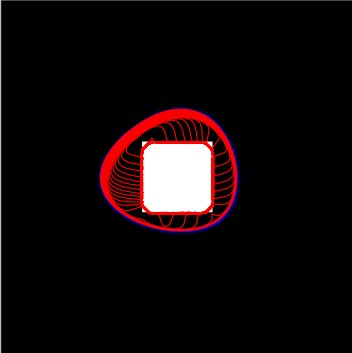
\includegraphics[width=\textwidth]{108}
                \caption{Black square}
                \label{fig:Blacksquare}
        \end{subfigure}%
        ~ %add desired spacing between images, e. g. ~, \quad, \qquad etc.
          %(or a blank line to force the subfigure onto a new line)
        \begin{subfigure}[b]{0.2\textwidth}
                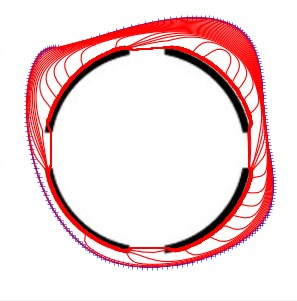
\includegraphics[width=\textwidth]{301}
                \caption{Gestalt circle}
                \label{fig:Gestaltcircle}
        \end{subfigure}
        ~ %add desired spacing between images, e. g. ~, \quad, \qquad etc.
          %(or a blank line to force the subfigure onto a new line)
        \begin{subfigure}[b]{0.2\textwidth}
                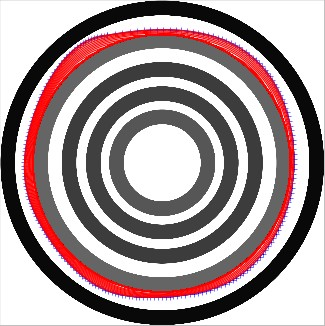
\includegraphics[width=\textwidth]{401}
                \caption{Many circles}
                \label{fig:Manycircles}
        \end{subfigure}
        \caption{Result images with $\alpha$=8,$\beta$=0,$\tau$=0.01,$\gamma$=500}\label{fig:resultimages}
\end{figure}
\

\section{Results}
Below are the images and the values($\alpha$, $\beta$, $\tau$, $\gamma$) used to produce them.\\


\begin{figure}[H]
        \centering
        \begin{subfigure}[b]{0.2\textwidth}
                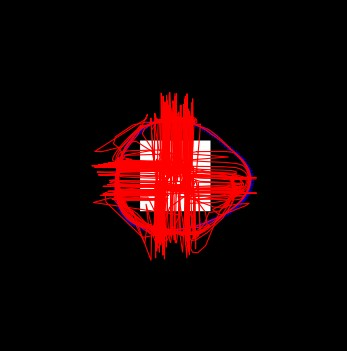
\includegraphics[width=\textwidth]{101}
                \caption{8,0,0.01,10000}
                \label{fig:Blacksquare1}
        \end{subfigure}%
        ~ %add desired spacing between images, e. g. ~, \quad, \qquad etc.
          %(or a blank line to force the subfigure onto a new line)
        \begin{subfigure}[b]{0.2\textwidth}
                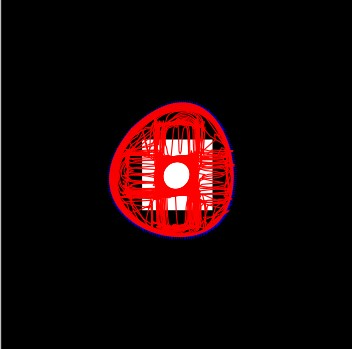
\includegraphics[width=\textwidth]{103}
                \caption{8,0,0.01,5000}
                \label{fig:Blacksquare2}
        \end{subfigure}
        ~ %add desired spacing between images, e. g. ~, \quad, \qquad etc.
          %(or a blank line to force the subfigure onto a new line)
        \begin{subfigure}[b]{0.2\textwidth}
                
\includegraphics[width=\textwidth]{105}
                \caption{8,0,0.01,1000}
                \label{fig:Blacksquare3}
        \end{subfigure}
         \begin{subfigure}[b]{0.2\textwidth}
                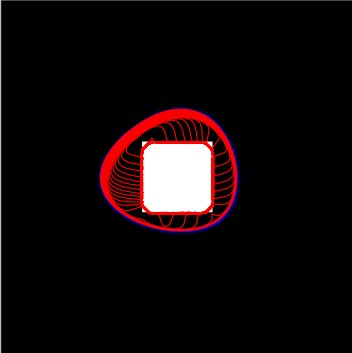
\includegraphics[width=\textwidth]{108}
                \caption{8,0,0.01,500}
                \label{fig:Blacksquare4}
        \end{subfigure}
        \caption{Result images series 1 }\label{fig:animals}
\end{figure}

\begin{figure}[H]
        \centering
        \begin{subfigure}[b]{0.2\textwidth}
                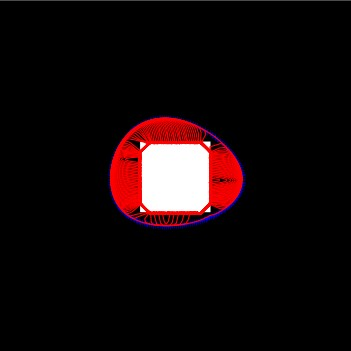
\includegraphics[width=\textwidth]{111}
                \caption{1,0,0.01,500}
                \label{fig:Blacksquare5}
        \end{subfigure}%
        ~ %add desired spacing between images, e. g. ~, \quad, \qquad etc.
          %(or a blank line to force the subfigure onto a new line)
        \begin{subfigure}[b]{0.2\textwidth}
                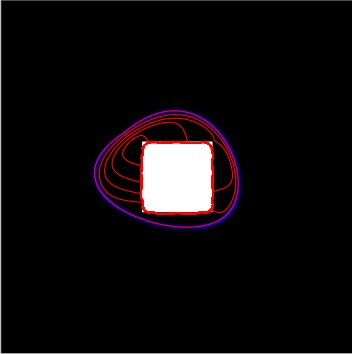
\includegraphics[width=\textwidth]{114}
                \caption{50,0,0.01,500}
                \label{fig:Blacksquare6}
        \end{subfigure}
        ~ %add desired spacing between images, e. g. ~, \quad, \qquad etc.
          %(or a blank line to force the subfigure onto a new line)
        \begin{subfigure}[b]{0.2\textwidth}
                
\includegraphics[width=\textwidth]{118}
                \caption{8,0,0.01,2}
                \label{fig:Blacksquare7}
        \end{subfigure}
         \begin{subfigure}[b]{0.2\textwidth}
                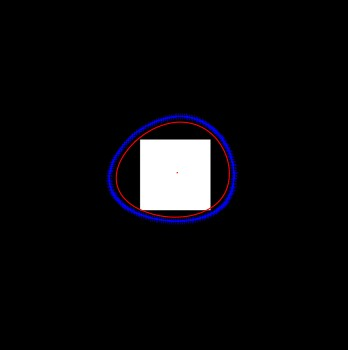
\includegraphics[width=\textwidth]{123}
                \caption{10000,0,0.01,500}
                \label{fig:Blacksquare8}
        \end{subfigure}
        \caption{Result images series 2}\label{fig:animals}
\end{figure}

\begin{figure}[H]
        \centering
        \begin{subfigure}[b]{0.2\textwidth}
                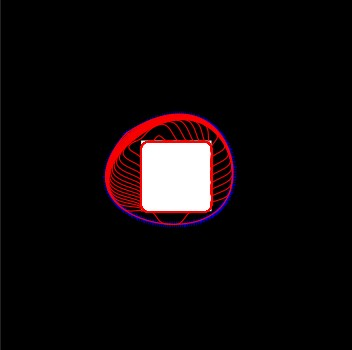
\includegraphics[width=\textwidth]{121}
                \caption{8,50,0.01,100}
                \label{fig:Blacksquare9}
        \end{subfigure}%
        ~ %add desired spacing between images, e. g. ~, \quad, \qquad etc.
          %(or a blank line to force the subfigure onto a new line)
        \begin{subfigure}[b]{0.2\textwidth}
                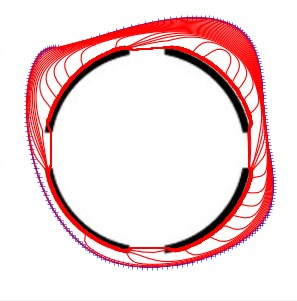
\includegraphics[width=\textwidth]{301}
                \caption{8,0,0.01,500}
                \label{fig:Gestaltcircle1}
        \end{subfigure}
        ~ %add desired spacing between images, e. g. ~, \quad, \qquad etc.
          %(or a blank line to force the subfigure onto a new line)
        \begin{subfigure}[b]{0.2\textwidth}
                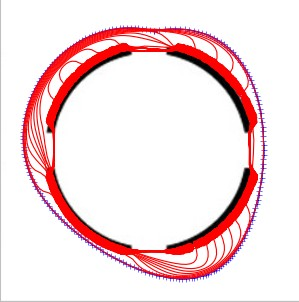
\includegraphics[width=\textwidth]{303}
                \caption{8,0,0.01,1000}
                \label{fig:Gestaltcircle2}
        \end{subfigure}
         \begin{subfigure}[b]{0.2\textwidth}
                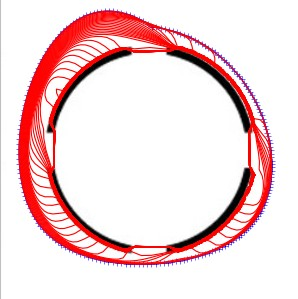
\includegraphics[width=\textwidth]{304}
                \caption{4,0,0.01,500}
                \label{fig:Gestaltcircle3}
        \end{subfigure}
        \caption{Result images series 3 }\label{fig:animals}
\end{figure}


\begin{figure}[H]
        \centering
        \begin{subfigure}[b]{0.2\textwidth}
                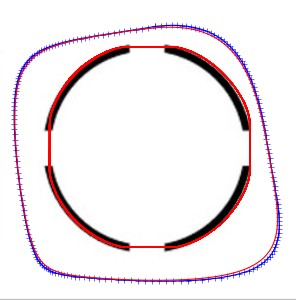
\includegraphics[width=\textwidth]{307}
                \caption{1000,0,0.01,500}
                \label{fig:Gestaltcircle4}
        \end{subfigure}%
        ~ %add desired spacing between images, e. g. ~, \quad, \qquad etc.
          %(or a blank line to force the subfigure onto a new line)
        \begin{subfigure}[b]{0.2\textwidth}
                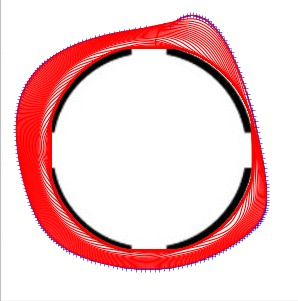
\includegraphics[width=\textwidth]{311}
                \caption{8,8,0.01,8}
                \label{fig:Gestaltcircle5}
        \end{subfigure}
        ~ %add desired spacing between images, e. g. ~, \quad, \qquad etc.
          %(or a blank line to force the subfigure onto a new line)
        \begin{subfigure}[b]{0.2\textwidth}
                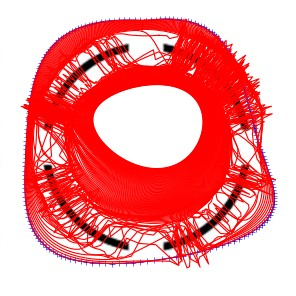
\includegraphics[width=\textwidth]{308}
                \caption{8,0,0.01,5000}
                \label{fig:Gestaltcircle6}
        \end{subfigure}
         \begin{subfigure}[b]{0.2\textwidth}
                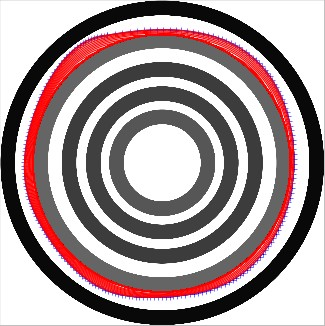
\includegraphics[width=\textwidth]{401}
                \caption{8,0,0.01,500}
                \label{fig:Manycircles1}
        \end{subfigure}
        \caption{Result images series 4 }\label{fig:animals}
\end{figure}

\begin{figure}[H]
        \centering
        \begin{subfigure}[b]{0.2\textwidth}
                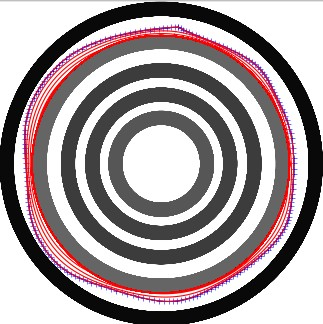
\includegraphics[width=\textwidth]{405}
                \caption{20,0,0.01,500}
                \label{fig:Manycircles2}
        \end{subfigure}%
        ~ %add desired spacing between images, e. g. ~, \quad, \qquad etc.
          %(or a blank line to force the subfigure onto a new line)
        \begin{subfigure}[b]{0.2\textwidth}
                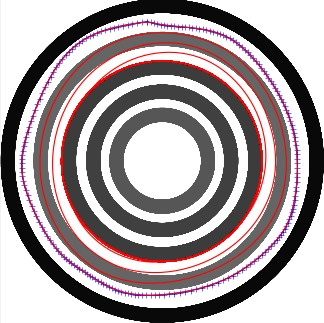
\includegraphics[width=\textwidth]{406}
                \caption{100,0,0.01,500}
                \label{fig:Manycircles3}
        \end{subfigure}
       
        \caption{Result images series 5 }\label{fig:animals}
\end{figure}

\

\section{Discussion}
\subsection{Black square}
\subsubsection{$\gamma$}
If the external energy, $\gamma$, is too strong (e.g. 5000), the snake is pulled violently towards any edge, but cannot hold on to it and may end inside the shape, see 1.1 and 1.3. We didn't find $\alpha$ values that could balance such high $\gamma$ values. When we lower $\gamma$, the edge becomes gradually less curly (Figure 5.1(c)) and at $\alpha$ = 8 and $\gamma$ 500 the edge is nice and smooth (Figure 5.1(d)).
\
\subsubsection{$\alpha$ and $\gamma$}
With $\gamma$ 500, both $\alpha$ 1 and 50 (and values between) produce nice images (Figure 5.2(a),(b)). $\alpha$ = 50 make it go to the edges of the shape in fewer iterations. $\gamma$ 2 (with $\alpha$ being 8) also produce a nice end result, but the lower the $\gamma$ is, the less forceful it is pulled towards the shape and it needs more steps to reach the edges of the shape (Figure 5.2(c)). If $\alpha$ is too high (10000) and $\gamma$ is 500 the internal force (which tries to minimize the surface tension) is stronger than the external force (which tries to make the snake follow the square) and the snake ends like a circle just outside the square (Figure 5.2(d)). This effect is for obvious reasons not visible for the circles.\\
\subsubsection{$\gamma$, $\alpha$ and $\beta$}
If we have $\alpha$ = 8 and $\gamma$ = 100 (pretty low) then a higher $\beta$ (50) can make the snake find the edge in fewer steps than with $\beta$ = 0 (Figure 5.3(a)). 
\
\subsection{Gestalt circle}
The gestalt circle seems like the easiest task for the snake. Because it is circular and there are no other shapes in the imge than a circle (though broken), most values find the edge; $\alpha$ 4 to 1000 and $\gamma$ 8 to 1000 produce nice shapes (Figure 5.3(b),(c),(d) and Figure 5.4(a),(b))  On most images it's visible that the snake is pulled towards the lines and not the gaps. Only with $\gamma$ 5000 the snake is pulled over the edges and ends inside the circle. (Figure 5.4(c)) 
\
\subsection{Many circles}
If $\gamma$ is 500 then $\alpha$ up to 20 make the snake attach to the light gray circle (Figure 5.4(d) and Figure 5.5(a)). Higher $\alpha$ values make the external force relatively weaker and it does not attach to the light gray circle anymore, but attaches to the first dark gray circle it meets. (Figure 5.5(b)). 
\end{document}